\documentclass[11pt]{report}

% Paquetes y configuraciones adicionales
\usepackage{graphicx}
\usepackage[export]{adjustbox}
\usepackage{caption}
\usepackage{float}
\usepackage{titlesec}
\usepackage{geometry}
\usepackage[hidelinks]{hyperref}
\usepackage{titling}
\usepackage{titlesec}
\usepackage{parskip}
\usepackage{wasysym}
\usepackage{tikzsymbols}
\usepackage{fancyvrb}
\usepackage{xurl}
\usepackage{hyperref}
\usepackage{subcaption}

\usepackage{listings}
\usepackage{xcolor}

\usepackage[spanish]{babel}

\newcommand{\subtitle}[1]{
  \posttitle{
    \par\end{center}
    \begin{center}\large#1\end{center}
    \vskip0.5em}
}

% Configura los márgenes
\geometry{
  left=2cm,   % Ajusta este valor al margen izquierdo deseado
  right=2cm,  % Ajusta este valor al margen derecho deseado
  top=3cm,
  bottom=3cm,
}

% Configuración de los títulos de las secciones
\titlespacing{\section}{0pt}{\parskip}{\parskip}
\titlespacing{\subsection}{0pt}{\parskip}{\parskip}
\titlespacing{\subsubsection}{0pt}{\parskip}{\parskip}

% Redefinir el formato de los capítulos y añadir un punto después del número
\makeatletter
\renewcommand{\@makechapterhead}[1]{%
  \vspace*{0\p@} % Ajusta este valor para el espaciado deseado antes del título del capítulo
  {\parindent \z@ \raggedright \normalfont
    \ifnum \c@secnumdepth >\m@ne
        \huge\bfseries \thechapter.\ % Añade un punto después del número
    \fi
    \interlinepenalty\@M
    #1\par\nobreak
    \vspace{10pt} % Ajusta este valor para el espacio deseado después del título del capítulo
  }}
\makeatother

% Configura para que cada \chapter no comience en una pagina nueva
\makeatletter
\renewcommand\chapter{\@startsection{chapter}{0}{\z@}%
    {-3.5ex \@plus -1ex \@minus -.2ex}%
    {2.3ex \@plus.2ex}%
    {\normalfont\Large\bfseries}}
\makeatother

% Configurar los colores para el código
\definecolor{codegreen}{rgb}{0,0.6,0}
\definecolor{codegray}{rgb}{0.5,0.5,0.5}
\definecolor{codepurple}{rgb}{0.58,0,0.82}
\definecolor{backcolour}{rgb}{0.95,0.95,0.92}

% Configurar el estilo para el código
\lstdefinestyle{mystyle}{
  backgroundcolor=\color{backcolour},   
  commentstyle=\color{codegreen},
  keywordstyle=\color{magenta},
  numberstyle=\tiny\color{codegray},
  stringstyle=\color{codepurple},
  basicstyle=\ttfamily\footnotesize,
  breakatwhitespace=false,         
  breaklines=true,                 
  captionpos=b,                    
  keepspaces=true,                 
  numbers=left,                    
  numbersep=5pt,                  
  showspaces=false,                
  showstringspaces=false,
  showtabs=false,                  
  tabsize=2
}

%==============================================================================
% Cosas para la documentación LateX
% % Sangría
% \setlength{\parindent}{1em}Texto

% % Quitar sangría
% \noindent

% % Punto
% \CIRCLE \ \ \textbf{Texto} \emph{algo}
% \begin{itemize}
%   \item \textbf{Negrita:} Texto
%   \item \textbf{Negrita:} Texto
% \end{itemize}

% % Introducir código
% \begin{center}
%   \begin{BVerbatim}
%     ... Código
%   \end{BVerbatim}
% \end{center}

% Poner una imagen
% \begin{figure}[H]
%   \centering
%   \includegraphics[scale=0.55]{img/}
%   \caption{Exportación de la base de datos en formato sql}
%   \label{fig:exportación de la base de datos en formato sql}
% \end{figure}

% Poner dos imágenes
% \begin{figure}[H]
%   \begin{subfigure}{0.5\textwidth}
%     \centering
%     \includegraphics[scale=0.45]{img/}
%     \caption{Texto imagen 1}
%   \end{subfigure}%
%   \begin{subfigure}{0.5\textwidth}
%     \centering
%     \includegraphics[scale=0.45]{img/}
%     \caption{Texto imagen 2}
%   \end{subfigure}
%   \caption{Texto general}
% \end{figure}

% % Poner una tabla
% \begin{table}[H]
%   \centering
%   \begin{tabular}{|c|c|c|c|}
%     \hline
%     \textbf{Campo 1} & \textbf{Campo 2} & \textbf{Campo 3} & \textbf{Campo 4} \\ \hline
%     Texto & Texto & Texto & Texto \\ \hline
%     Texto & Texto & Texto & Texto \\ \hline
%     Texto & Texto & Texto & Texto \\ \hline
%     Texto & Texto & Texto & Texto \\ \hline
%   \end{tabular}
%   \caption{Nombre de la tabla}
%   \label{tab:nombre de la tabla}
% \end{table}

% % Poner codigo de un lenguaje a partir de un archivo
% \lstset{style=mystyle}
% The next code will be directly imported from a file
% \lstinputlisting[language=Python]{code.py}

% “Texto entre comillas dobles”

%==============================================================================

\begin{document}

% Portada del informe
\title{Practica 12. Pentesting con Metasploit}
\subtitle{Seguridad de Sistemas Informáticos}
\author{Carlos Pérez Fino \texttt{alu0101340333@ull.edu.es} \and Cheuk Kelly Ng Pante \texttt{alu0101364544@ull.edu.es}}
\date{\today}

\maketitle

\pagestyle{empty} % Desactiva la numeración de página para el índice

% Índice
\tableofcontents

% Nueva página
\cleardoublepage

\pagestyle{plain} % Vuelve a activar la numeración de página
\setcounter{page}{1} % Reinicia el contador de página a 1

% Secciones del informe
% Capitulo 1
\chapter{Instalación de Kali Linux y Metasploitable 2}
Para esta práctica se ha instalado Kali Linux en una máquina virtual y Metasploitable 2 en otra máquina virtual. Ambas máquinas se han instalado en VirtualBox. Para la configuración 
de la red se ha utilizado la opcion de “Redes Nat” para que ambas máquinas puedan comunicarse entre ellas. Para la configuración de la red lo que hay que hacer es en VirtualBox ir a:
\begin{verbatim}
Archivo -> Herramientas -> Administrador de red -> Redes Nat
\end{verbatim}

y ahi crear una nueva red Nat.
\begin{figure}[H]
  \centering
  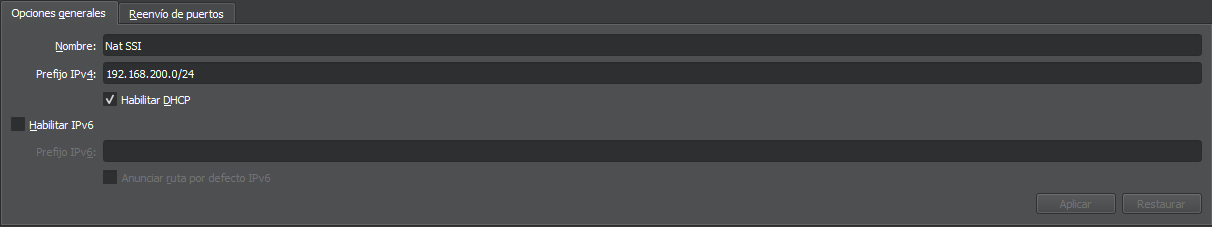
\includegraphics[scale=0.5]{img/red_nat.png}
  \caption{Creación de una nueva red Nat}
  \label{fig:Creación de una nueva red Nat}
\end{figure}

Una vez creada la red Nat, hay que ir a la configuración de cada máquina virtual y en la pestaña de “Red” seleccionar en el apartado “Conectados” \texttt{->} “Red Nat” y por defecto saldra la
red que se ha creado anteriormente.

\begin{figure}[H]
  \begin{subfigure}{0.5\textwidth}
    \centering
    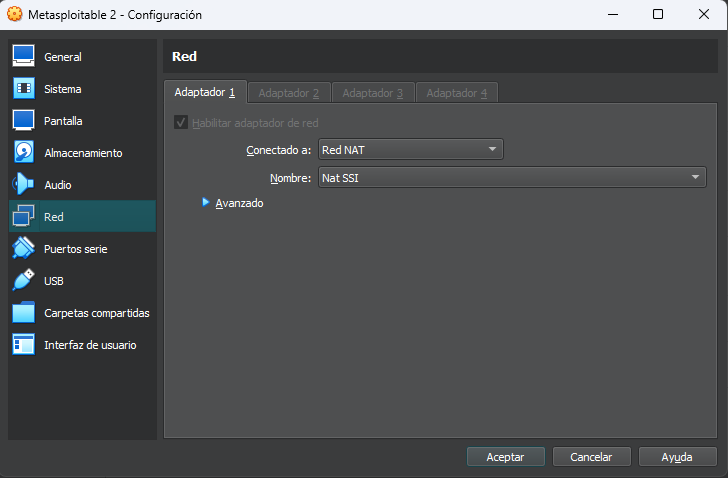
\includegraphics[scale=0.45]{img/red_nat_mv.png}
    \caption{Configuración de la red Nat en la MV}
  \end{subfigure}%
  \begin{subfigure}{0.5\textwidth}
    \centering
    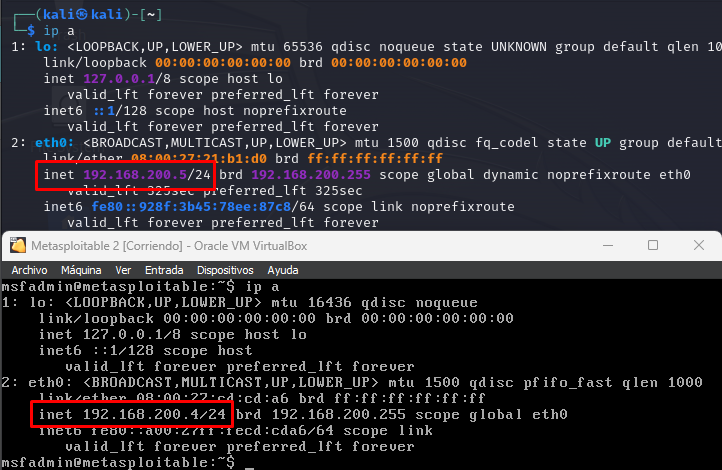
\includegraphics[scale=0.46]{img/red_nat_set.png}
    \caption{IPs de las máquinas virtuales}
  \end{subfigure}
  \caption{Configuración de la red Nat}
\end{figure}

\newpage

% Capitulo 2
\chapter{Vulnerabilidades de Metasploitable 2}
% 2.1
\section{nmap}
Para realizar un escaneo de puertos con nmap, primero hay que saber la IP de la máquina virtual de Metasploitable 2. Una vez sabida la IP, se ejecuta el siguiente comando en la máquina Kali:
\begin{verbatim}
nmap 192.168.200.4 --top-ports 100 -sV
\end{verbatim}

Al ejecutar el comando anterior se va a obtener una lista de los puertos abiertos y los servicios que se están ejecutando en cada puerto. En la siguiente imagen se puede ver el resultado del comando anterior.
\begin{figure}[H]
  \centering
  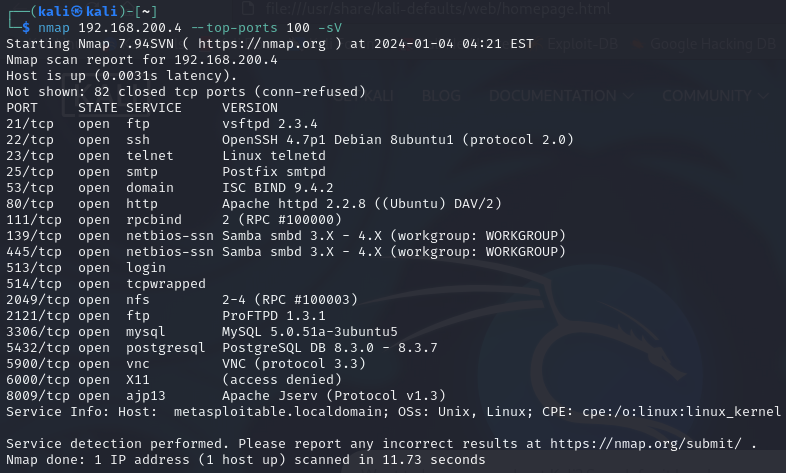
\includegraphics[scale=0.55]{img/nmap.png}
  \caption{Resultado del comando nmap}
  \label{fig:Resultado del comando nmap}
\end{figure}

% 2.2
% \section{ftp}
% Para realizar un ataque de fuerza bruta con ftp primero hay que saber el usuario que se va a atacar. Para ello se ejecuta el siguiente comando en la máquina Kali:
% \begin{verbatim}
% nmap
% \end{verbatim}

% Al ejecutar el comando anterior se va a obtener una lista de los puertos abiertos y los servicios que se están ejecutando en cada puerto. En la siguiente imagen se puede ver el resultado del comando anterior.
% \begin{figure}[H]
%   \centering
%   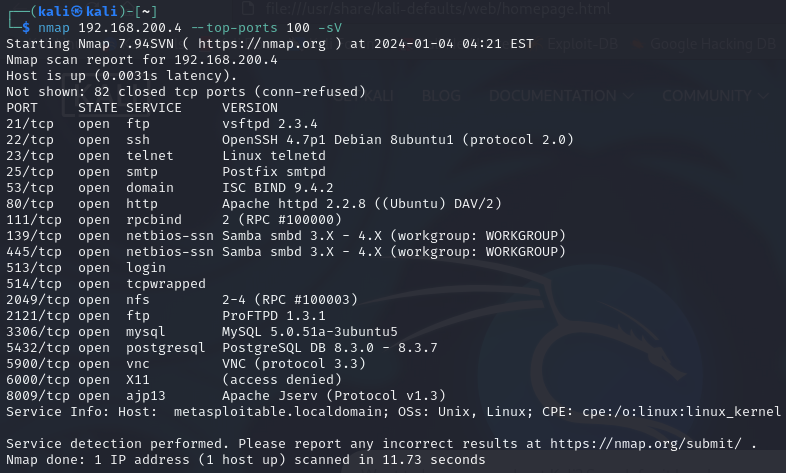
\includegraphics[scale=0.5]{img/nmap.png}
%   \caption{Resultado del comando nmap}
% \end{figure}

% Una vez sabido el usuario, se ejecuta el siguiente comando en la máquina Kali:
% \begin{verbatim}
% hydra -l msfadmin -P /usr/share/wordlists/rockyou.txt

% ftp://192.168.200.4
% \end{verbatim}

% Al ejecutar el comando anterior se va a obtener la contraseña del usuario msfadmin. En la siguiente imagen se puede ver el resultado del comando anterior.
% \begin{figure}[H]
%   \centering
%   \includegraphics[scale=0.5]{img/hydra_ftp.png}
%   \caption{Resultado del comando hydra}
% \end{figure}

% 2.3
\section{Exploit de vsftpd 2.3.4}
Para realizar un ataque de fuerza bruta con ftp vamos a obtener con el comando \emph{nmap} la versión del servicio ftp que se está ejecutando en el puerto 21.
Una vez tenemos la versión del servicio ftp, vamos a buscar un exploit para esa versión. Para ellos, entramos en la consola del Framework Metasploit con el comando \emph{msfconsole} y ejecutamos el siguiente comando:
\begin{BVerbatim}
search vsftpd 2.3.4
\end{BVerbatim}

Una vez encontrado el exploit, vamos a configurarlo con el comando \emph{use} y el nombre del exploit o poniendo el id del exploit.
\begin{figure}[H]
  \centering
  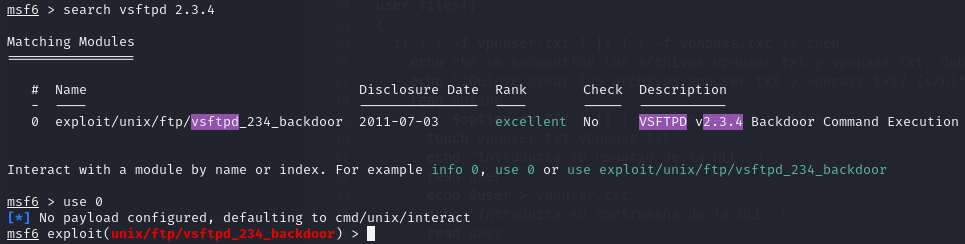
\includegraphics[scale=0.5]{img/search_vsftpd.png}
  \caption{Resultado del comando search}
\end{figure}

Una vez seleccionado el exploit, vamos a usar \emph{options} para ver las opciones que tiene el exploit y vamos a configurar el exploit en las opciones donde la columna indica \emph{required} y \emph{yes} con el comando 
\emph{set} y el nombre de la opción y el valor que queremos ponerle a esa opción.
\begin{verbatim}
set RHOST 192.168.200.4
set RPORT 21
\end{verbatim}

\begin{figure}[H]
  \centering
  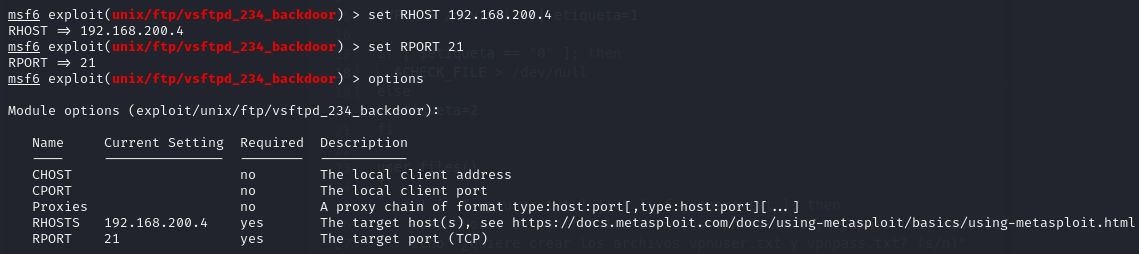
\includegraphics[scale=0.51]{img/options_vsftpd.png}
  \caption{Resultado del comando options}
\end{figure}

Una vez configurado el exploit, vamos a ejecutarlo con el comando \emph{run} y vamos a obtener una shell de la máquina de Metasploitable 2.
\begin{figure}[H]
  \centering
  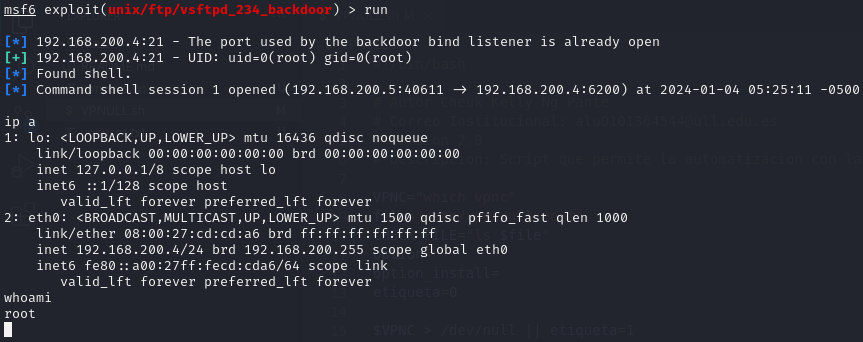
\includegraphics[scale=0.6]{img/run_vsftpd.png}
  \caption{Resultado del comando run}
\end{figure}

\chapter{Exploit puerto 22 – SSH}

\newpage

\chapter{Bibliografía} % En formato APA
\begin{thebibliography}{99}
  \bibitem{0} Kali Linux. (2023). Kali Linux. \url{https://cdimage.kali.org/kali-2023.4/kali-linux-2023.4-virtualbox-amd64.7z}
  \bibitem{1} Gandia, K. (2023). METASPLOITABLE 2 Descargar e Instalar en VirtualBox + Tutorial Vulnerabilidad FTP. \url{https://www.youtube.com/watch?v=x0Pj0rIV_Mk}
  \bibitem{2} Natário, R. (2020). Metasploitable 3 Ubuntu Walkthrough: Part II. \url{https://tremblinguterus.blogspot.com/2020/11/metasploitable-3-ubuntu-walkthrough_10.html}
  \bibitem{3} Núñez Marín, J. M. (2022). RESOLUCIÓN DE METASPLOITABLE 2. \url{https://elhackeretico.com/resolucion-de-metasploitable-2/}
\end{thebibliography}

\end{document}
